\appendix
\section{Anhang}
\begin{table}[h]
  \centering
  \begin{tabular}{S S}
    \toprule
    {$\nu\:/\:\si{\kilo\hertz}$} & {$\overline{U_\text{a}^2}\:/\:\si{\volt\squared}$}\\
    \midrule
    1.127 & 0.373\\
1.09 & 0.336\\
1.181 & 0.398\\
1.223 & 0.419\\
1.274 & 0.438\\
1.298 & 0.447\\
1.324 & 0.455\\
1.34 & 0.459\\
1.404 & 0.471\\
1.484 & 0.479\\
1.653 & 0.485\\
1.942 & 0.486\\
2.2 & 0.479\\
2.312 & 0.481\\
2.638 & 0.478\\
2.749 & 0.476\\
2.924 & 0.474\\
3.115 & 0.469\\
3.493 & 0.466\\
3.76 & 0.464\\
3.959 & 0.463\\
4.48 & 0.463\\
5.935 & 0.46\\
6.89 & 0.461\\
7.876 & 0.462\\
8.823 & 0.46\\
9.85 & 0.46\\
10.862 & 0.462\\
15.801 & 0.46\\
25.363 & 0.455\\
26.6 & 0.451\\

    \bottomrule
  \end{tabular}
  \begin{tabular}{S S}
    \toprule
    {$\nu\:/\:\si{\kilo\hertz}$} & {$\overline{U_\text{a}^2}\:/\:\si{\volt\squared}$}\\
    \midrule
    27.732 & 0.44\\
    28.078 & 0.436\\
    28.645 & 0.433\\
    29.443 & 0.429\\
    31.3 & 0.425\\
    31.923 & 0.424\\
    32.993 & 0.422\\
    34.093 & 0.411\\
    34.846 & 0.404\\
    35.663 & 0.395\\
    36.265 & 0.39\\
    37.033 & 0.385\\
    37.698 & 0.379\\
    38.466 & 0.371\\
    39.012 & 0.363\\
    39.36 & 0.357\\
    40.098 & 0.344\\
    41.097 & 0.329\\
    41.588 & 0.32\\
    41.7 & 0.319\\
    42.29 & 0.308\\
    42.741 & 0.298\\
    43.6 & 0.284\\
    44.81 & 0.263\\
    45.879 & 0.237\\
    46.708 & 0.222\\
    47.862 & 0.201\\
    48.408 & 0.192\\
    48.89 & 0.183\\
    49.835 & 0.17\\
    50.196 & 0.161\\
  \bottomrule
\end{tabular}
  \caption{Messwerte der Durchlasskurve für die einfache Schaltung.}
  \label{tab:durchlasseinfach}
\end{table}

\begin{table}[h]
  \centering
  \begin{tabular}[t]{S S S}
    \toprule
    {$\nu\:/\:\si{\kilo\hertz}$} & {$\overline{U_\text{a}^2}\:/\:\si{\volt\squared}$} & {$V_N$}\\
    \midrule
    0.342 & 0.051 & 20\\
    0.512 & 0.117 & 20\\
    0.604 & 0.165 & 20\\
    0.667 & 0.203 & 20\\
    0.773 & 0.278 & 20\\
    0.814 & 0.31 & 20\\
    0.89 & 0.376 & 20\\
    0.942 & 0.424 & 20\\
    1.023 & 0.509 & 20\\
    1.086 & 0.582 & 20\\
    1.126 & 0.635 & 20\\
    1.141 & 0.66 & 20\\
    1.184 & 0.724 & 20\\
    1.232 & 0.779 & 20\\
    1.294 & 0.872 & 20\\
    1.321 & 0.915 & 20\\
    1.349 & 0.969 & 20\\
    1.401 & 1.035 & 20\\
    1.481 & 1.19 & 20\\
    1.506 & 1.275 & 20\\
    1.606 & 1.5 & 20\\
    1.664 & 1.65 & 20\\
    1.73 & 1.875 & 20\\
    1.754 & 1.92 & 20\\
    1.81 & 2.05 & 20\\
    1.863 & 2.2 & 20\\
    1.92 & 2.45 & 20\\
    1.972 & 2.63 & 20\\
    1.978 & 2.8 & 20\\
    2.046 & 3.05 & 20\\
    2.129 & 3.4 & 20\\
    2.196 & 3.74 & 20\\
    2.225 & 4.22 & 20\\
    2.304 & 4.55 & 20\\
    2.383 & 5.25 & 20\\
    2.438 & 5.3 & 20\\

    \bottomrule
  \end{tabular}
  \begin{tabular}[t]{S S S}
    \toprule
    {$\nu\:/\:\si{\kilo\hertz}$} & {$\overline{U_\text{a}^2}\:/\:\si{\volt\squared}$} & {$V_N$}\\
    \midrule

    2.487 & 4.52 & 20\\
    2.539 & 4.81 & 20\\
    2.569 & 4.93 & 20\\
    2.633 & 5.32 & 20\\
    2.696 & 5.74 & 20\\
    2.744 & 6.11 & 20\\
    2.821 & 6.78 & 20\\
    2.936 & 7.9 & 20\\
    3.021 & 8.9 & 20\\
    3.108 & 2.38 & 10\\
    3.217 & 2.76 & 10\\
    3.358 & 3.45 & 10\\
    3.478 & 4.01 & 10\\
    3.637 & 5.32 & 10\\
    3.722 & 6.18 & 10\\
    3.757 & 6.55 & 10\\
    3.86 & 7.9 & 10\\
    3.924 & 8.84 & 10\\
    4.001 & 2.69 & 5\\
    4.264 & 4.93 & 5\\
    4.349 & 6.35 & 5\\
    4.475 & 9.18 & 5\\
    4.568 & 2.1 & 2\\
    4.683 & 3.16 & 2\\
    4.75 & 4.0 & 2\\
    4.811 & 5.1 & 2\\
    4.933 & 7.7 & 2\\
    5.038 & 8.64 & 2\\
    5.12 & 7.85 & 2\\
    5.215 & 6.25 & 2\\
    5.33 & 4.2 & 2\\
    5.446 & 2.8 & 2\\
    5.596 & 1.84 & 2\\
    5.706 & 1.38 & 2\\
    5.901 & 5.6 & 5\\
  \bottomrule
\end{tabular}
\begin{tabular}[t]{S S S}
  \toprule
  {$\nu\:/\:\si{\kilo\hertz}$} & {$\overline{U_\text{a}^2}\:/\:\si{\volt\squared}$} & {$V_N$}\\
  \midrule

  6.033 & 4.41 & 5\\
  6.17 & 3.51 & 5\\
  6.231 & 3.2 & 5\\
  6.32 & 2.77 & 5\\
  6.474 & 2.29 & 5\\
  6.58 & 2.06 & 5\\
  6.651 & 1.89 & 5\\
  6.827 & 6.04 & 10\\
  6.928 & 5.57 & 10\\
  7.042 & 5.01 & 10\\
  7.208 & 4.34 & 10\\
  7.349 & 3.94 & 10\\
  7.472 & 3.6 & 10\\
  7.64 & 3.2 & 10\\
  7.776 & 2.96 & 10\\
  8.044 & 2.57 & 10\\
  8.245 & 2.23 & 10\\
  8.433 & 2.02 & 10\\
  8.664 & 1.8 & 10\\
  8.87 & 7.07 & 20\\
  8.98 & 6.74 & 20\\
  9.167 & 6.25 & 20\\
  9.357 & 5.81 & 20\\
  9.671 & 5.22 & 20\\
  9.939 & 4.76 & 20\\
  10.37 & 4.22 & 20\\
  11.769 & 2.8 & 20\\
  13.206 & 1.85 & 20\\
  14.901 & 1.45 & 20\\
  17.841 & 0.92 & 20\\
  21.065 & 0.63 & 20\\
  26.828 & 0.36 & 20\\
  38.231 & 0.172 & 20\\
  53.018 & 0.085 & 20\\
  65.861 & 0.049 & 20\\
  \bottomrule
\end{tabular}
  \caption{Messwerte der Durchlasskurve für die Korrelatorschaltung.}
  \label{tab:durchlasskorr}
\end{table}

\begin{table}
  \centering
  \begin{tabular}{S S S}
    \toprule
    {$R\:/\:\si{\ohm}$} & {$\overline{U_\text{a}^2}\:/\:\si{\volt\squared}$} & {$V_N$}\\
    \midrule
105 & 0.191 & 50\\
200 & 0.623 & 50\\
300 & 1.282 & 50\\
400 & 2.08 & 50\\
499 & 0.492 & 20\\
599 & 0.646 & 20\\
701 & 0.82 & 20\\
800 & 0.988 & 20\\
900 & 1.161 & 20\\
995 & 1.325 & 20\\
    \bottomrule
  \end{tabular}
  \caption{Messwerte vom thermischen Rauschen des Widerstands $R_1$ bei einfacher Schaltung.}
  \label{tab:widerstand1}
\end{table}

\begin{table}
  \centering
  \begin{tabular}{S S S}
    \toprule
    {$R\:/\:\si{\kilo\ohm}$} & {$\overline{U_\text{a}^2}\:/\:\si{\volt\squared}$} & {$V_N$}\\
    \midrule
    2 & 0.12 & 100\\
    4 & 0.08 & 50\\
    6 & 0.1 & 50\\
    8 & 0.14 & 50\\
    10 & 0.17 & 50\\
    12 & 0.205 & 50\\
    14 & 0.245 & 50\\
    16 & 0.28 & 50\\
    18 & 0.3 & 50\\
    20 & 0.335 & 50\\
    \bottomrule
  \end{tabular}
  \caption{Messwerte vom thermischen Rauschen des Widerstands $R_2$ bei einfacher Schaltung.}
  \label{tab:widerstand2}
\end{table}

\begin{table}
  \centering
  \begin{tabular}{S S S}
    \toprule
    {$R\:/\:\si{\ohm}$} & {$\overline{U_\text{a}^2}\:/\:\si{\volt\squared}$} & {$V_N$}\\
    \midrule
    100.1 & 0.19 & 500\\
    202 & 0.475 & 500\\
    301 & 0.76 & 500\\
    400 & 1.04 & 500\\
    500 & 0.219 & 200\\
    601 & 0.265 & 200\\
    700 & 0.305 & 200\\
    800 & 0.355 & 200\\
    900 & 0.405 & 200\\
    995 & 0.445 & 200\\
    \bottomrule
  \end{tabular}
  \caption{Messwerte vom thermischen Rauschen des Widerstands $R_1$ mit Korrelatorschaltung.}
  \label{tab:widerstand1korr}
\end{table}

\begin{table}
  \centering
  \begin{tabular}{S S S}
    \toprule
    {$R\:/\:\si{\kilo\ohm}$} & {$\overline{U_\text{a}^2}\:/\:\si{\volt\squared}$} & {$V_N$}\\
    \midrule
    2.0 & 1.01 & 200\\
    4.1 & 1.92 & 200\\
    6.08 & 0.68 & 100\\
    7.99 & 0.88 & 100\\
    9.96 & 1.1 & 100\\
    11.94 & 1.33 & 100\\
    14.01 & 1.57 & 100\\
    15.98 & 1.74 & 100\\
    18.02 & 0.5 & 50\\
    19.9 & 0.56 & 50\\
    \bottomrule
  \end{tabular}
  \caption{Messwerte vom thermischen Rauschen des Widerstands $R_2$ mit Korrelatorschaltung.}
  \label{tab:widerstand2korr}
\end{table}

\begin{table}
  \centering
  \begin{tabular}{S S}
    \toprule
    {$I_\text{anode}\:/\:\si{\milli\ampere}$} & {$\overline{U_\text{anode}}\:/\:\si{\volt}$}\\
    \midrule
    0.4 & 10\\
    0.4 & 20\\
    0.4 & 30\\
    0.4 & 40\\
    0.4 & 45\\
    0.4 & 65\\
    0.5 & 85\\
    0.5 & 100\\
    0.5 & 120\\
    0.5 & 140\\
    0.5 & 155\\
    0.5 & 185\\
    \bottomrule
  \end{tabular}
  \caption{Messwerte der Kennlinie der Hochvakuumdiode mit Reinmetallkathode bei $I_\text{heiz} = \SI{0.9}{\ampere}$.}
  \label{tab:kennlinie1}
\end{table}
\begin{table}
  \centering
  \begin{tabular}{S S}
    \toprule
    {$I_\text{anode}\:/\:\si{\milli\ampere}$} & {$\overline{U_\text{anode}}\:/\:\si{\volt}$}\\
    \midrule
    1.1 & 10\\
    2.1 & 20\\
    2.3 & 30\\
    2.4 & 40\\
    2.4 & 45\\
    2.5 & 65\\
    2.5 & 85\\
    2.5 & 100\\
    2.5 & 120\\
    2.6 & 135\\
    2.6 & 155\\
    2.6 & 185\\
    \bottomrule
  \end{tabular}
  \caption{Messwerte der Kennlinie der Hochvakuumdiode mit Reinmetallkathode bei $I_\text{heiz} = \SI{1}{\ampere}$.}
  \label{tab:kennlinie2}
\end{table}
\begin{table}
  \centering
  \begin{tabular}{S S}
    \toprule
    {$I_\text{anode}\:/\:\si{\milli\ampere}$} & {$\overline{U_\text{anode}}\:/\:\si{\volt}$}\\
    \midrule
    0.9 & 10\\
    1.1 & 20\\
    1.1 & 30\\
    1.2 & 40\\
    1.2 & 45\\
    1.2 & 65\\
    1.2 & 85\\
    1.2 & 100\\
    1.3 & 120\\
    1.3 & 135\\
    1.3 & 155\\
    1.3 & 185\\
    \bottomrule
  \end{tabular}
  \caption{Messwerte der Kennlinie der Hochvakuumdiode mit Reinmetallkathode bei $I_\text{heiz} = \SI{0.95}{\ampere}$.}
  \label{tab:kennlinie3}
\end{table}
\begin{table}
  \centering
  \begin{tabular}{S S S}
    \toprule
    {$I_\text{anode}\:/\:\si{\milli\ampere}$} & {$\overline{U_\text{a}^2}\:/\:\si{\volt\squared}$} & {$V_\text{N}$}\\
    \midrule
    0.5 & 0.851 & 50\\
1.0 & 1.882 & 50\\
1.5 & 2.83 & 50\\
2.0 & 0.62 & 20\\
2.5 & 0.78 & 20\\
3.0 & 0.93 & 20\\
3.5 & 1.08 & 20\\
4.0 & 1.25 & 20\\
    \bottomrule
  \end{tabular}
  \caption{Messwerte zur Bestimmung der Elementarladung an der Reinmetallkathode. Die Fehler sind $\sigma_I = \SI{0.1}{\milli\ampere}$, $\sigma_{U^2} = \SI{0.05}{\volt\squared}$}
  \label{tab:elementar}
\end{table}
\begin{table}
  \centering
  \begin{tabular}{S[table-format=3.2]@{${}\pm{}$} S[table-format=2.3] S[table-format=2.3]@{${}\pm{}$} S[table-format=1.4]S[table-format=1.3]@{${}\pm{}$} S[table-format=1.3] S[table-format=4.0]}
    \toprule
    \multicolumn{2}{c}{$\nu_\text{m}\:/\:\si{\kilo\hertz}$} &\multicolumn{2}{c}{$\Delta_{\nu}\:/\:\si{\kilo\hertz}$}& \multicolumn{2}{c}{$\overline{U_\text{a}^2}\:/\:\si{\volt\squared}$} & {$V_\text{N}$}\\
    \midrule
    460.0 & 5.0 & 21.5 & 0.4 & 1.95 & 0.05 & 100\\
    440.0 & 5.0 & 23.0 & 0.4 & 2.28 & 0.05 & 100\\
    400.0 & 5.0 & 24.3 & 0.4 & 2.46 & 0.05 & 100\\
    360.0 & 5.0 & 24.4 & 0.4 & 2.73 & 0.05 & 100\\
    320.0 & 5.0 & 24.0 & 0.4 & 2.75 & 0.05 & 100\\
    300.0 & 5.0 & 23.4 & 0.4 & 3.08 & 0.05 & 100\\
    260.0 & 5.0 & 20.6 & 0.2 & 3.0 & 0.05 & 100\\
    240.0 & 5.0 & 20.9 & 0.2 & 2.89 & 0.05 & 100\\
    220.0 & 5.0 & 21.0 & 0.2 & 0.87 & 0.05 & 50\\
    200.0 & 5.0 & 18.8 & 0.0 & 0.786 & 0.05 & 50\\
    160.0 & 5.0 & 14.4 & 0.0 & 0.707 & 0.05 & 50\\
    140.0 & 5.0 & 13.0 & 0.0 & 0.651 & 0.05 & 50\\
    120.0 & 5.0 & 11.6 & 0.0 & 0.618 & 0.05 & 50\\
    100.0 & 10.0 & 12.1 & 1.09 & 0.75 & 0.005 & 50\\
    80.0 & 8.0 & 9.92 & 0.872 & 0.637 & 0.005 & 50\\
    60.0 & 6.0 & 7.74 & 0.654 & 0.5 & 0.005 & 50\\
    40.0 & 4.0 & 5.45 & 0.54 & 0.35 & 0.005 & 50\\
    20.0 & 2.0 & 2.75 & 0.27 & 0.699 & 0.005 & 100\\
    10.0 & 1.0 & 1.4 & 0.135 & 0.355 & 0.005 & 100\\
    8.0 & 0.8 & 1.127 & 0.112 & 0.282 & 0.005 & 100\\
    6.0 & 0.6 & 0.847 & 0.084 & 0.92 & 0.005 & 200\\
    4.0 & 0.4 & 0.567 & 0.056 & 0.585 & 0.005 & 200\\
    2.0 & 0.2 & 0.287 & 0.028 & 0.299 & 0.005 & 200\\
    1.0 & 0.1 & 0.147 & 0.014 & 0.885 & 0.005 & 500\\
    0.8 & 0.08 & 0.119 & 0.0112 & 0.725 & 0.005 & 500\\
    0.6 & 0.06 & 0.091 & 0.0084 & 0.565 & 0.005 & 500\\
    0.4 & 0.04 & 0.063 & 0.0056 & 0.263 & 0.005 & 500\\
    0.2 & 0.02 & 0.035 & 0.0028 & 0.175 & 0.005 & 500\\
    0.1 & 0.01 & 0.021 & 0.0014 & 0.11 & 0.005 & 500\\
    0.08 & 0.008 & 0.009 & 0.0012 & 0.38 & 0.005 & 1000\\
    0.06 & 0.006 & 0.006 & 0.0009 & 0.36 & 0.005 & 1000\\
    0.04 & 0.004 & 0.003 & 0.0006 & 0.31 & 0.005 & 1000\\
    \bottomrule
  \end{tabular}
  \caption{Messwerte, die für das Rauschspektrum der Hochvakuumdiode mit Reinmetallkathode aufgenommen wurden.}
  \label{tab:rauschspektrumrein}
\end{table}

\begin{table}
  \centering
  \begin{tabular}{S[table-format=3.2]@{${}\pm{}$} S[table-format=2.3] S[table-format=2.3]@{${}\pm{}$} S[table-format=1.4]S[table-format=1.3]@{${}\pm{}$} S[table-format=1.3] S[table-format=4.0]}
    \toprule
    \multicolumn{2}{c}{$\nu_\text{m}\:/\:\si{\kilo\hertz}$} &\multicolumn{2}{c}{$\Delta_{\nu}\:/\:\si{\kilo\hertz}$}& \multicolumn{2}{c}{$\overline{U_\text{a}^2}\:/\:\si{\volt\squared}$} & {$V_\text{N}$}\\
    \midrule
    460.0 & 5.0 & 34.3 & 0.2 & 0.222 & 0.05 & 20\\
    440.0 & 5.0 & 35.2 & 0.2 & 0.265 & 0.05 & 20\\
    400.0 & 5.0 & 34.8 & 0.2 & 0.239 & 0.05 & 20\\
    380.0 & 5.0 & 35.6 & 0.2 & 0.245 & 0.05 & 20\\
    360.0 & 5.0 & 35.2 & 0.3 & 0.237 & 0.05 & 20\\
    340.0 & 5.0 & 33.5 & 0.5 & 1.52 & 0.05 & 50\\
    320.0 & 5.0 & 33.0 & 0.5 & 1.49 & 0.05 & 50\\
    300.0 & 5.0 & 29.5 & 0.3 & 1.288 & 0.05 & 50\\
    280.0 & 5.0 & 27.5 & 0.5 & 1.17 & 0.05 & 50\\
    260.0 & 5.0 & 24.5 & 0.4 & 1.178 & 0.05 & 50\\
    240.0 & 5.0 & 24.8 & 0.4 & 1.154 & 0.05 & 50\\
    220.0 & 5.0 & 23.6 & 0.2 & 1.195 & 0.05 & 50\\
    200.0 & 5.0 & 21.5 & 0.2 & 1.03 & 0.05 & 50\\
    180.0 & 5.0 & 18.5 & 0.0 & 0.832 & 0.05 & 50\\
    160.0 & 5.0 & 16.3 & 0.0 & 0.74 & 0.05 & 50\\
    140.0 & 5.0 & 14.4 & 0.0 & 0.67 & 0.05 & 50\\
    120.0 & 5.0 & 12.2 & 0.0 & 0.594 & 0.05 & 50\\
    100.0 & 10.0 & 12.55 & 1.15 & 0.73 & 0.005 & 50\\
    80.0 & 8.0 & 10.25 & 0.92 & 0.6 & 0.005 & 50\\
    60.0 & 6.0 & 7.95 & 0.69 & 0.48 & 0.005 & 50\\
    40.0 & 4.0 & 5.45 & 0.54 & 0.313 & 0.005 & 50\\
    20.0 & 2.0 & 2.75 & 0.27 & 0.164 & 0.005 & 50\\
    10.0 & 1.0 & 1.4 & 0.135 & 1.45 & 0.005 & 200\\
    8.0 & 0.8 & 1.127 & 0.112 & 1.24 & 0.005 & 200\\
    6.0 & 0.6 & 0.847 & 0.084 & 1.01 & 0.005 & 200\\
    4.0 & 0.4 & 0.567 & 0.056 & 0.76 & 0.005 & 200\\
    2.0 & 0.2 & 0.287 & 0.028 & 0.525 & 0.005 & 200\\
    1.0 & 0.1 & 0.147 & 0.014 & 0.425 & 0.005 & 200\\
    0.8 & 0.08 & 0.119 & 0.0112 & 0.385 & 0.005 & 200\\
    0.6 & 0.06 & 0.091 & 0.0084 & 0.366 & 0.005 & 200\\
    0.4 & 0.04 & 0.063 & 0.0056 & 0.353 & 0.005 & 200\\
    0.2 & 0.02 & 0.035 & 0.0028 & 0.348 & 0.005 & 200\\
    0.1 & 0.01 & 0.021 & 0.0014 & 2.3 & 0.005 & 500\\
    0.08 & 0.008 & 0.009 & 0.0012 & 2.28 & 0.005 & 500\\
    0.06 & 0.006 & 0.006 & 0.0009 & 2.2 & 0.005 & 500\\
    0.04 & 0.004 & 0.003 & 0.0006 & 2.26 & 0.005 & 500\\
    \bottomrule
  \end{tabular}
  \caption{Messwerte, die für das Rauschspektrum der Hochvakuumdiode mit Oxidkathode aufgenommen wurden.}
  \label{tab:rauschspektrumoxid}
\end{table}



\section{Kopie der Originaldaten}

\begin{figure}
  \centering
  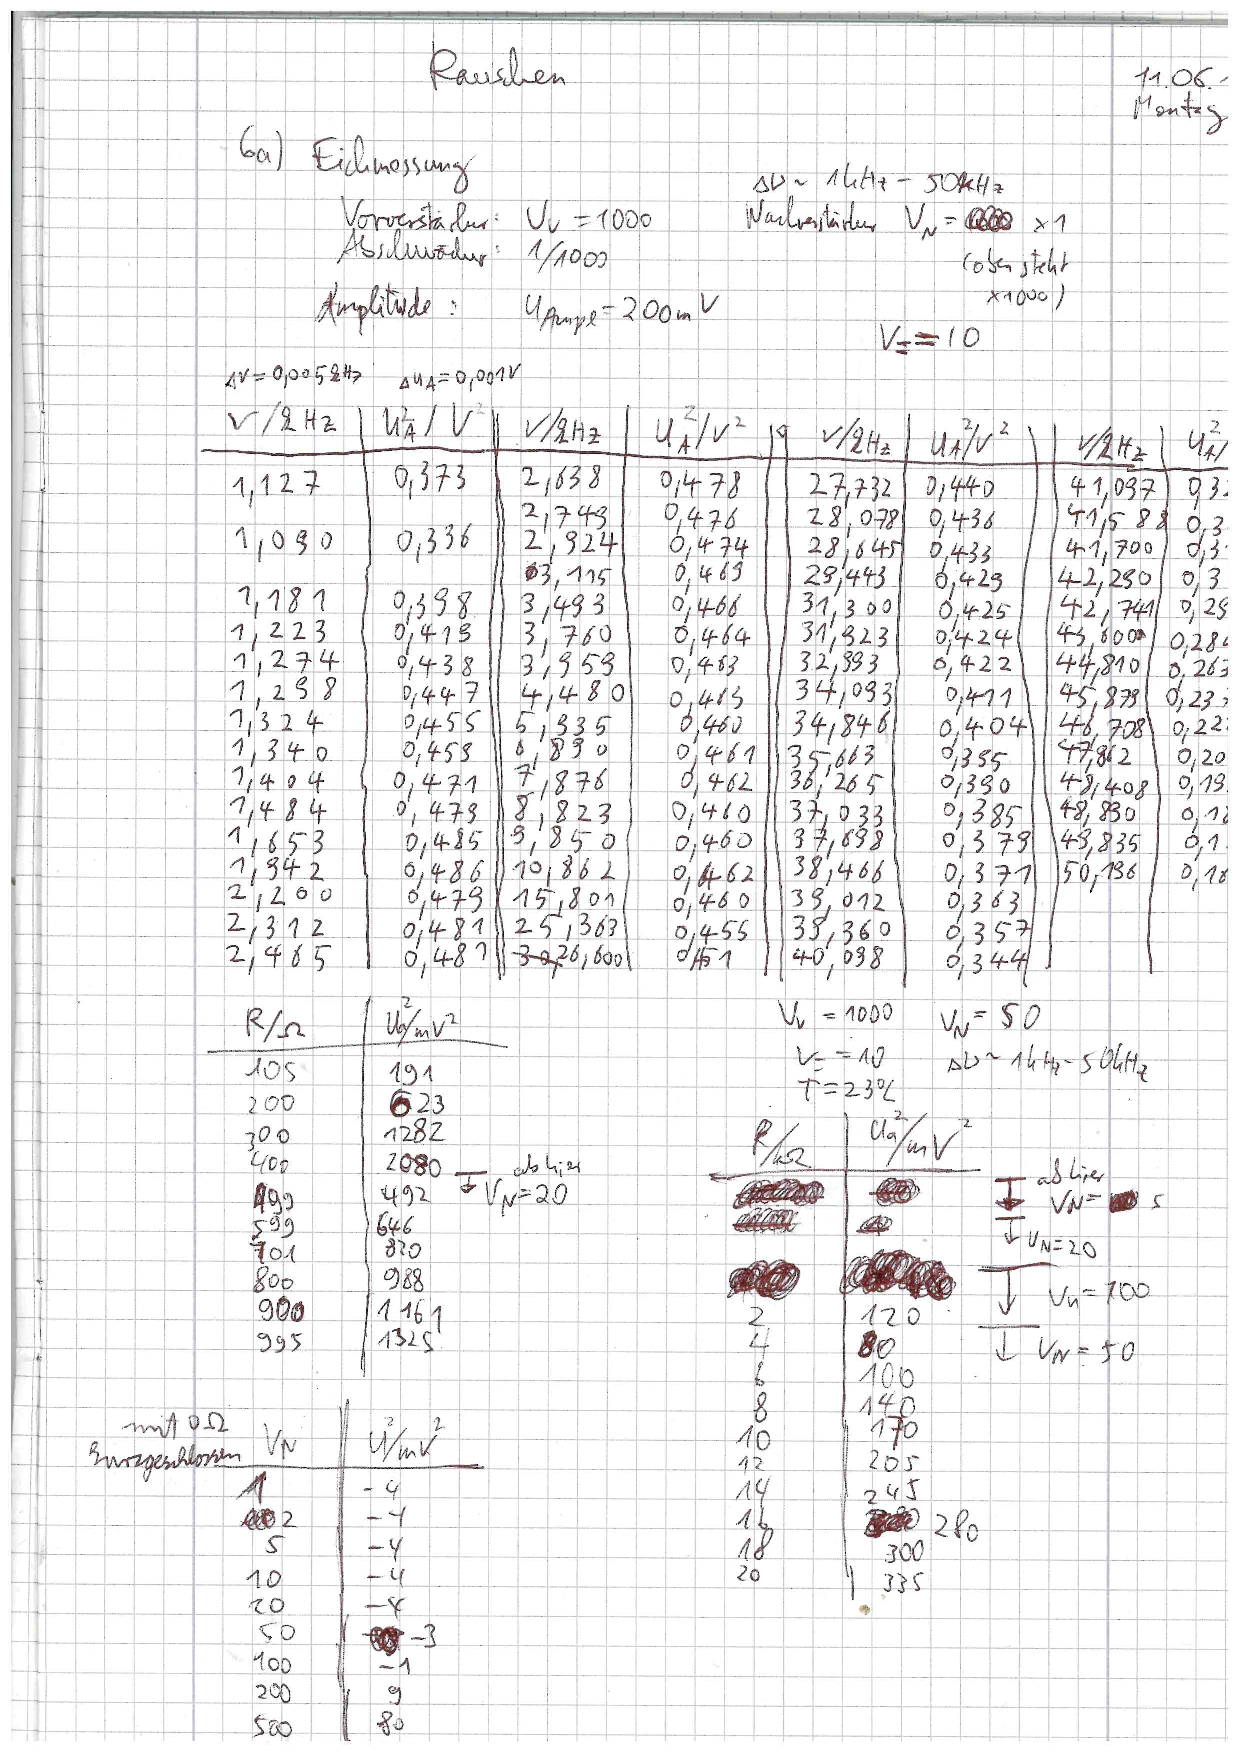
\includegraphics[width=0.8\textwidth]{messwerte/1.pdf}
  \caption{Erste Seite der Messwerte.}
  \label{fig:messwert1}
\end{figure}
\begin{figure}
  \centering
  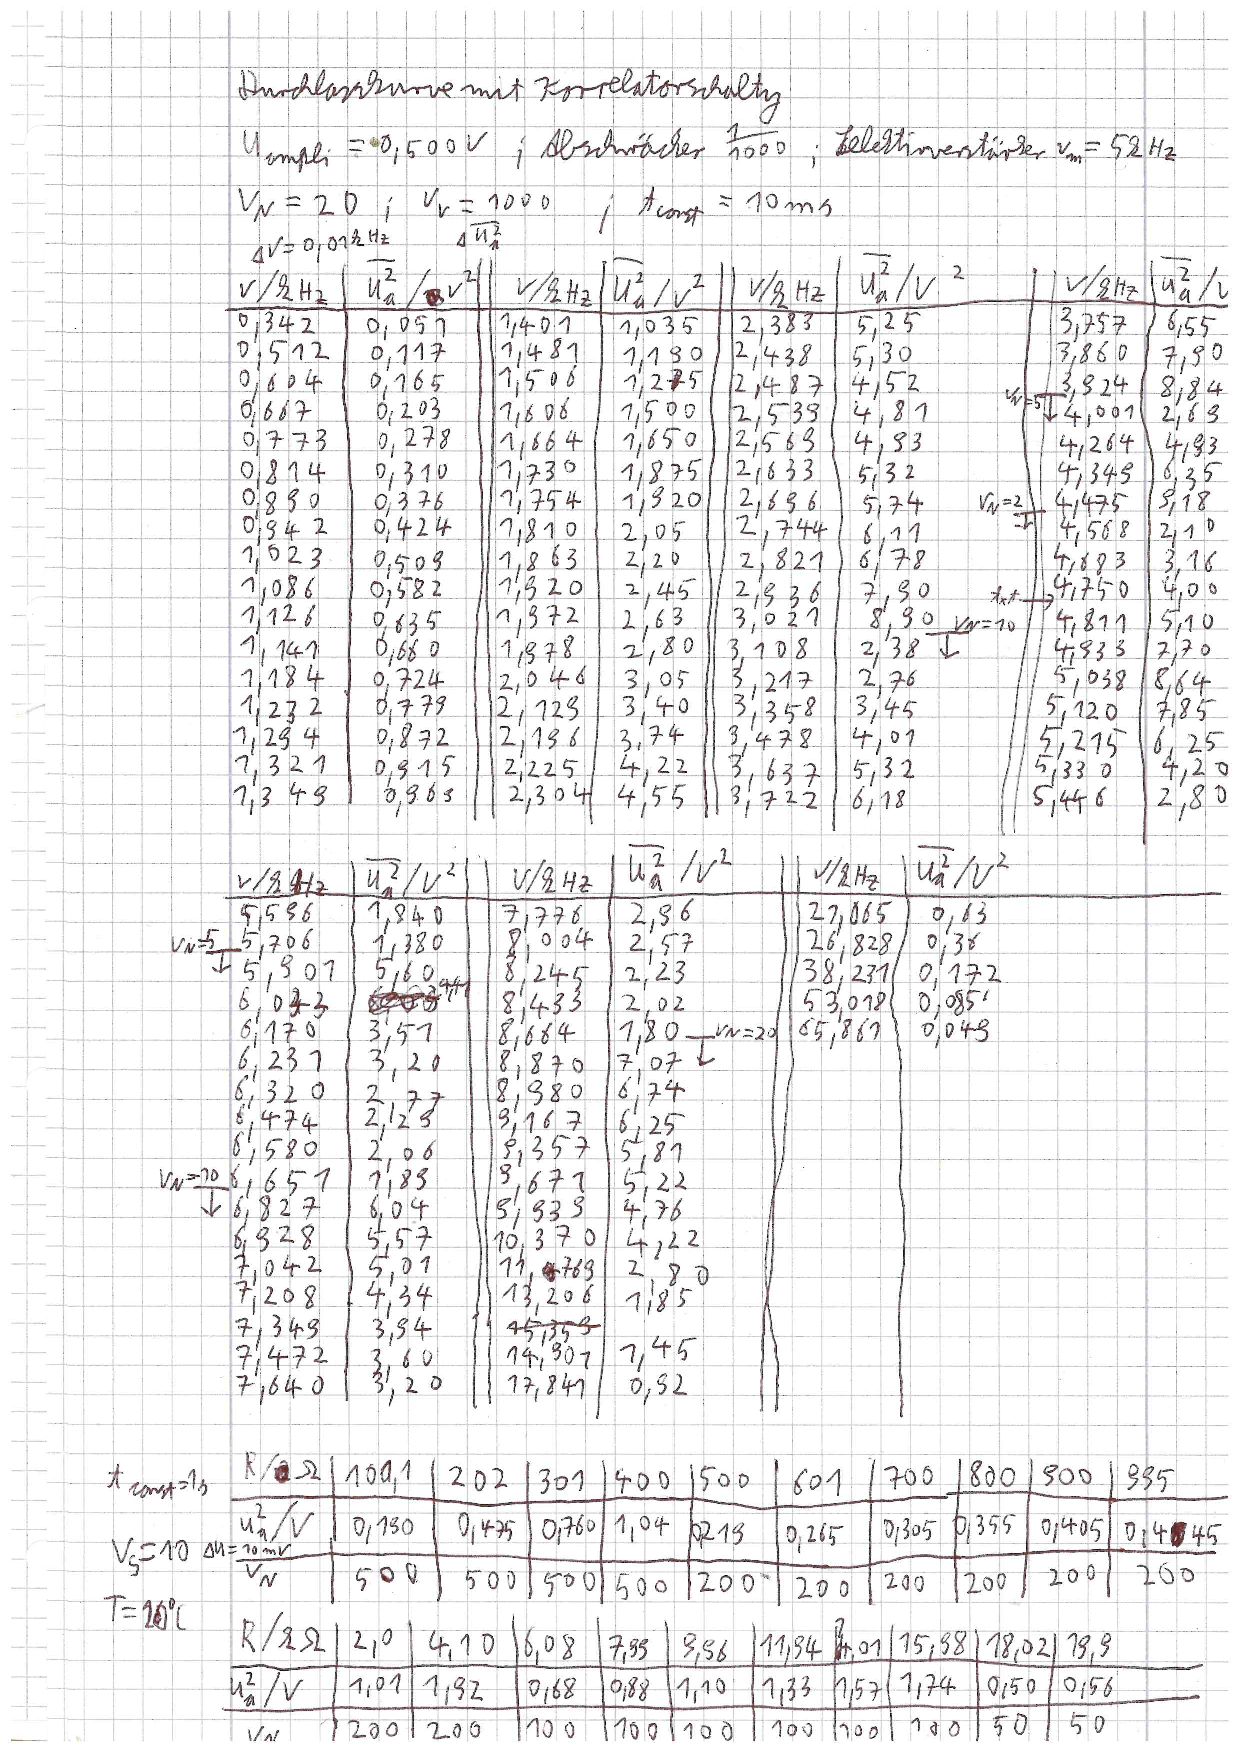
\includegraphics[width=0.8\textwidth]{messwerte/2.pdf}
  \caption{Zweite Seite der Messwerte.}
  \label{fig:messwert2}
\end{figure}
\begin{figure}
  \centering
  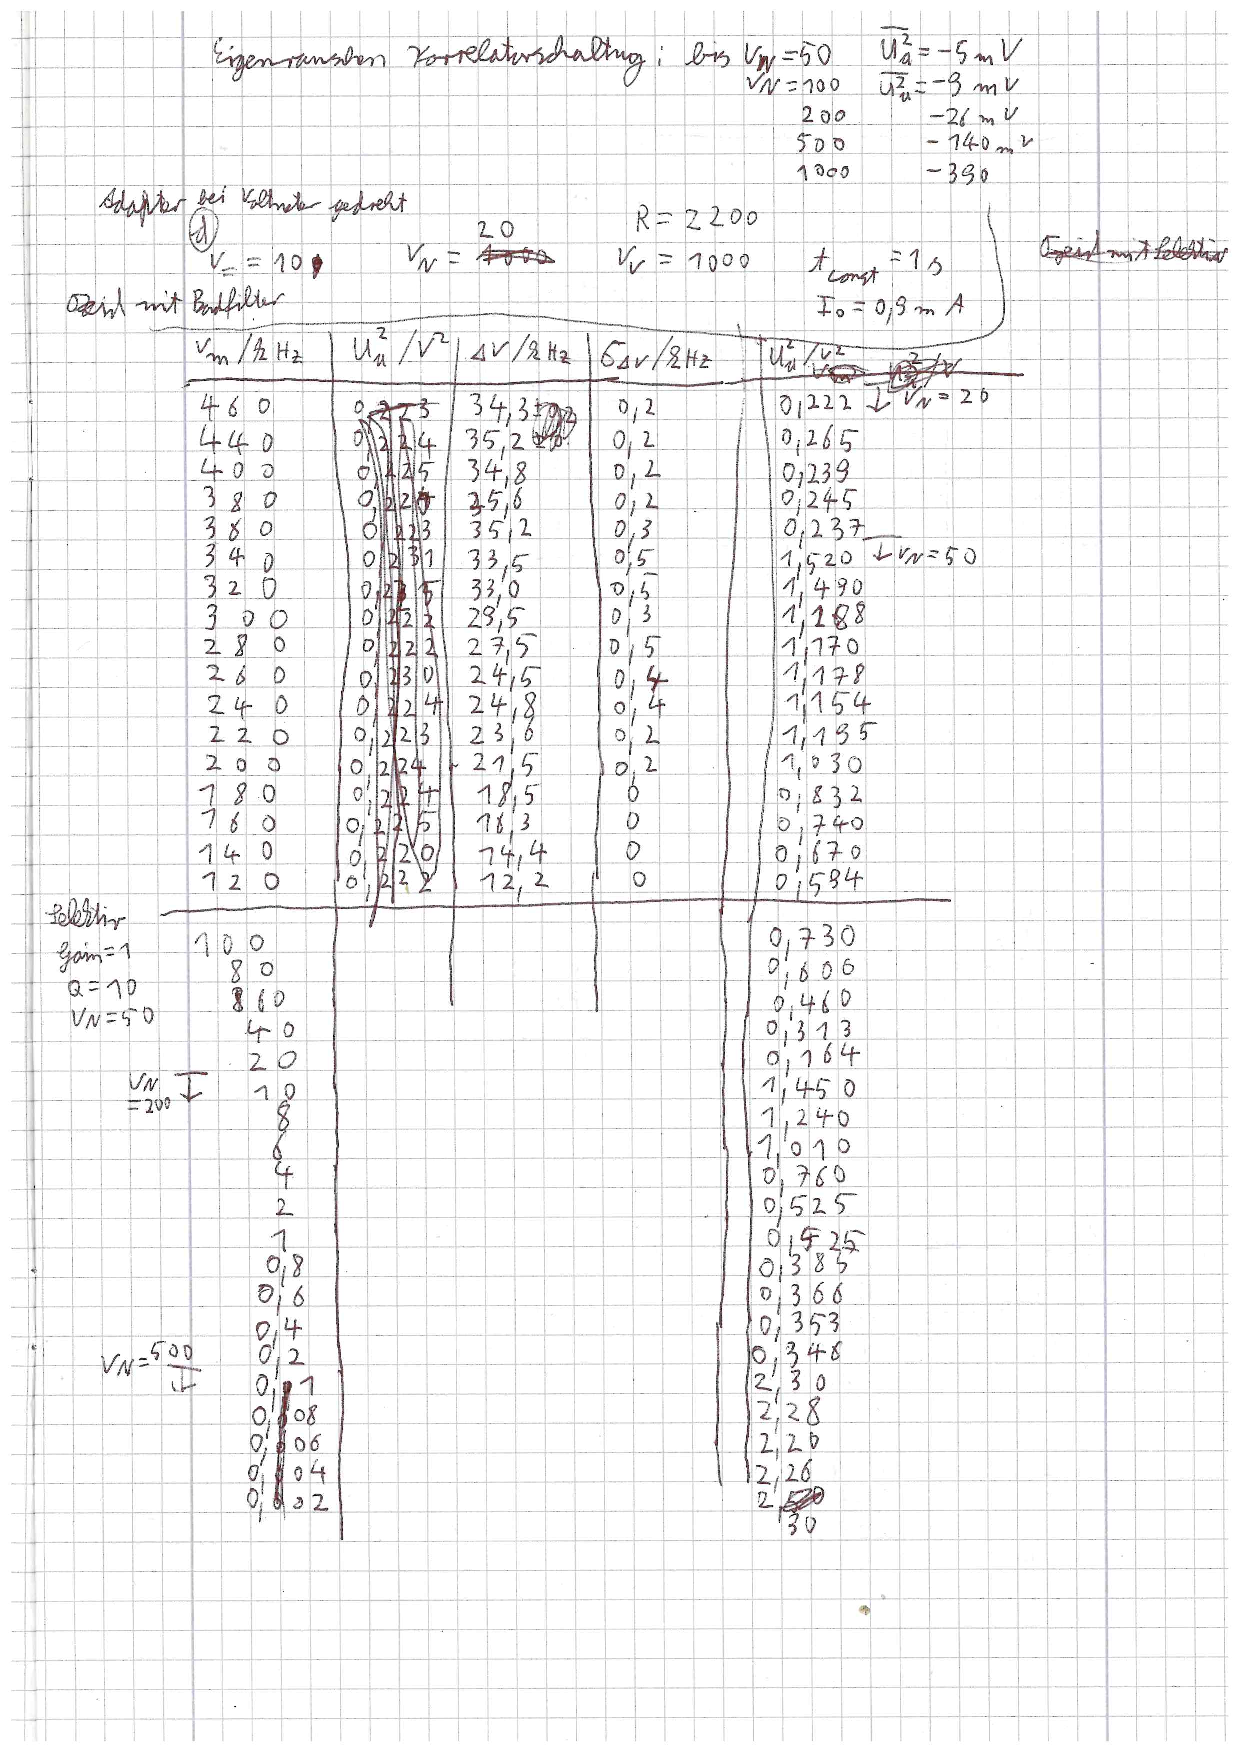
\includegraphics[width=0.8\textwidth]{messwerte/3.pdf}
  \caption{Dritte Seite der Messwerte.}
  \label{fig:messwert3}
\end{figure}
\begin{figure}
  \centering
  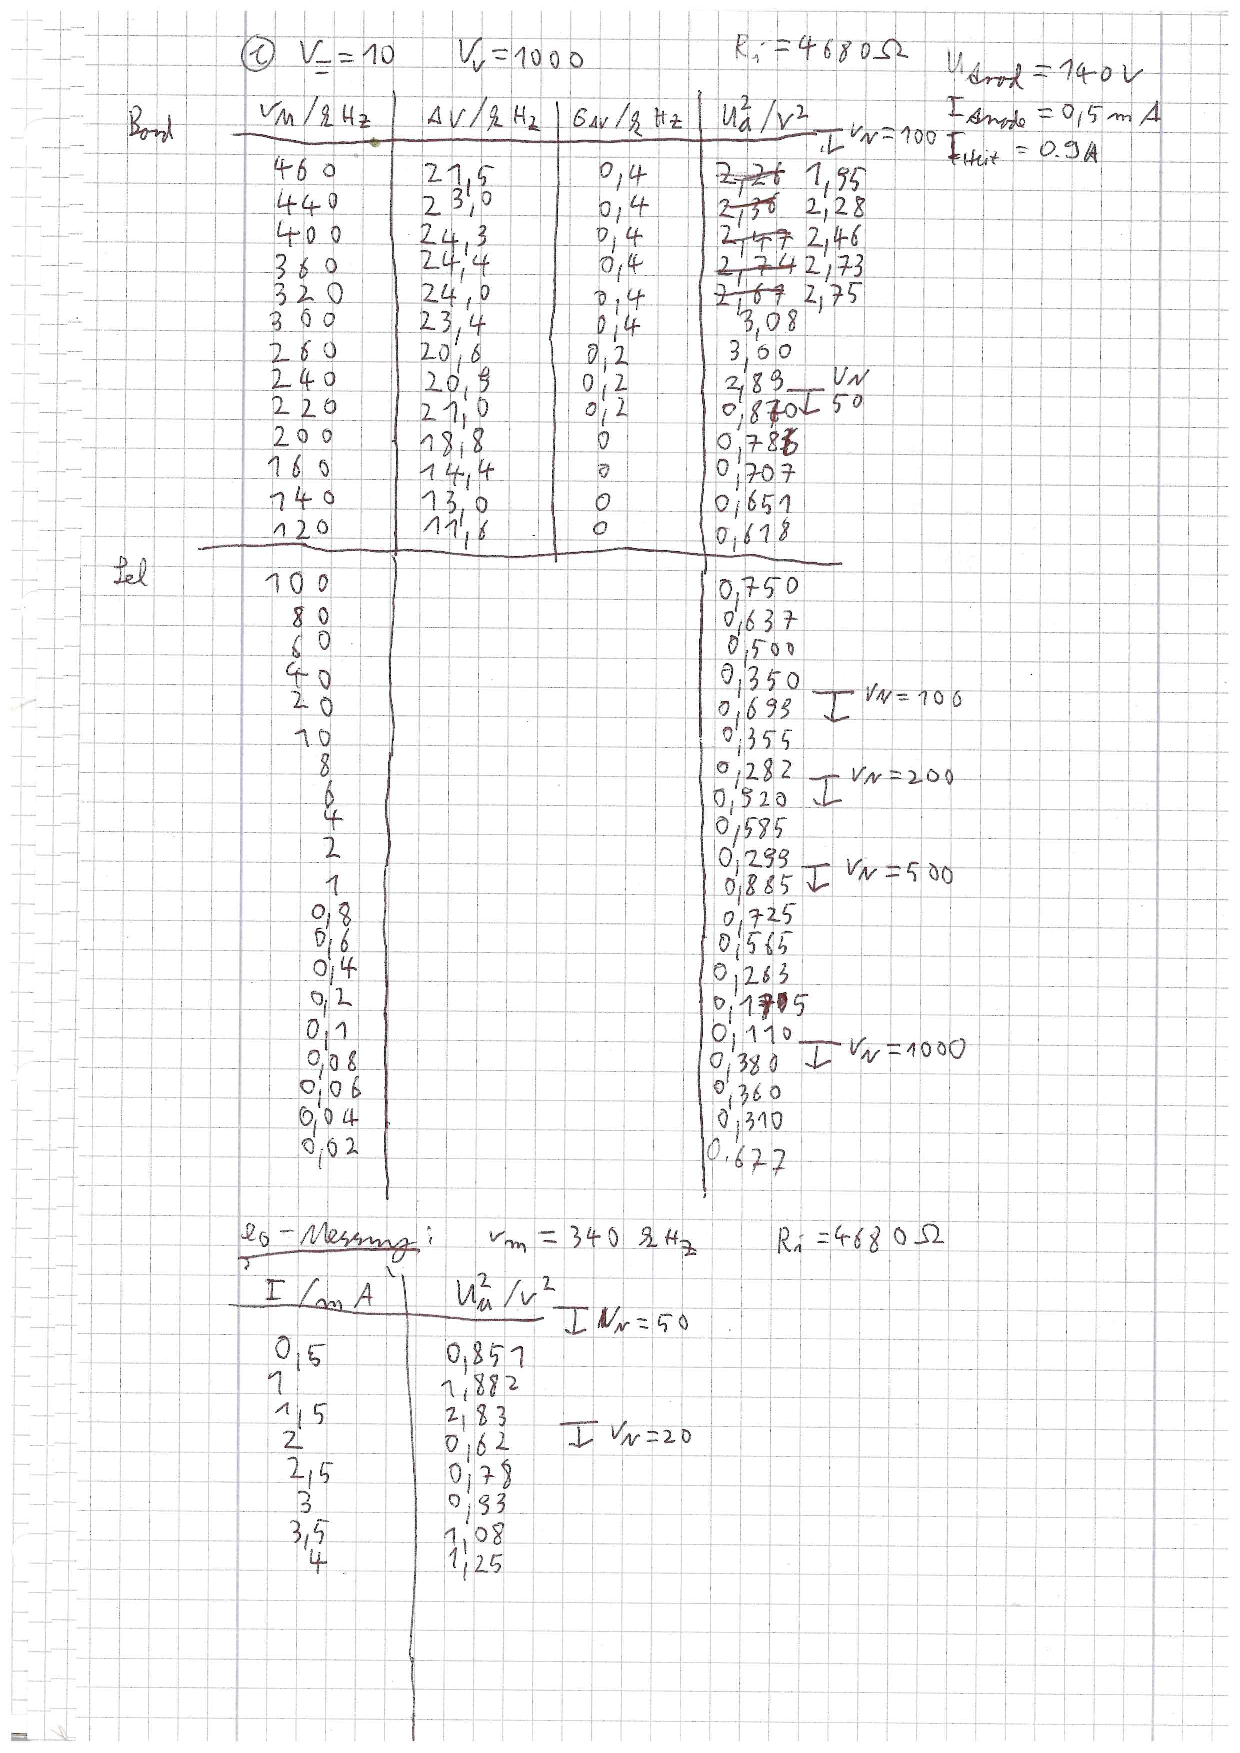
\includegraphics[width=0.8\textwidth]{messwerte/4.pdf}
  \caption{Vierte Seite der Messwerte.}
  \label{fig:messwert4}
\end{figure}
\begin{figure}
  \centering
  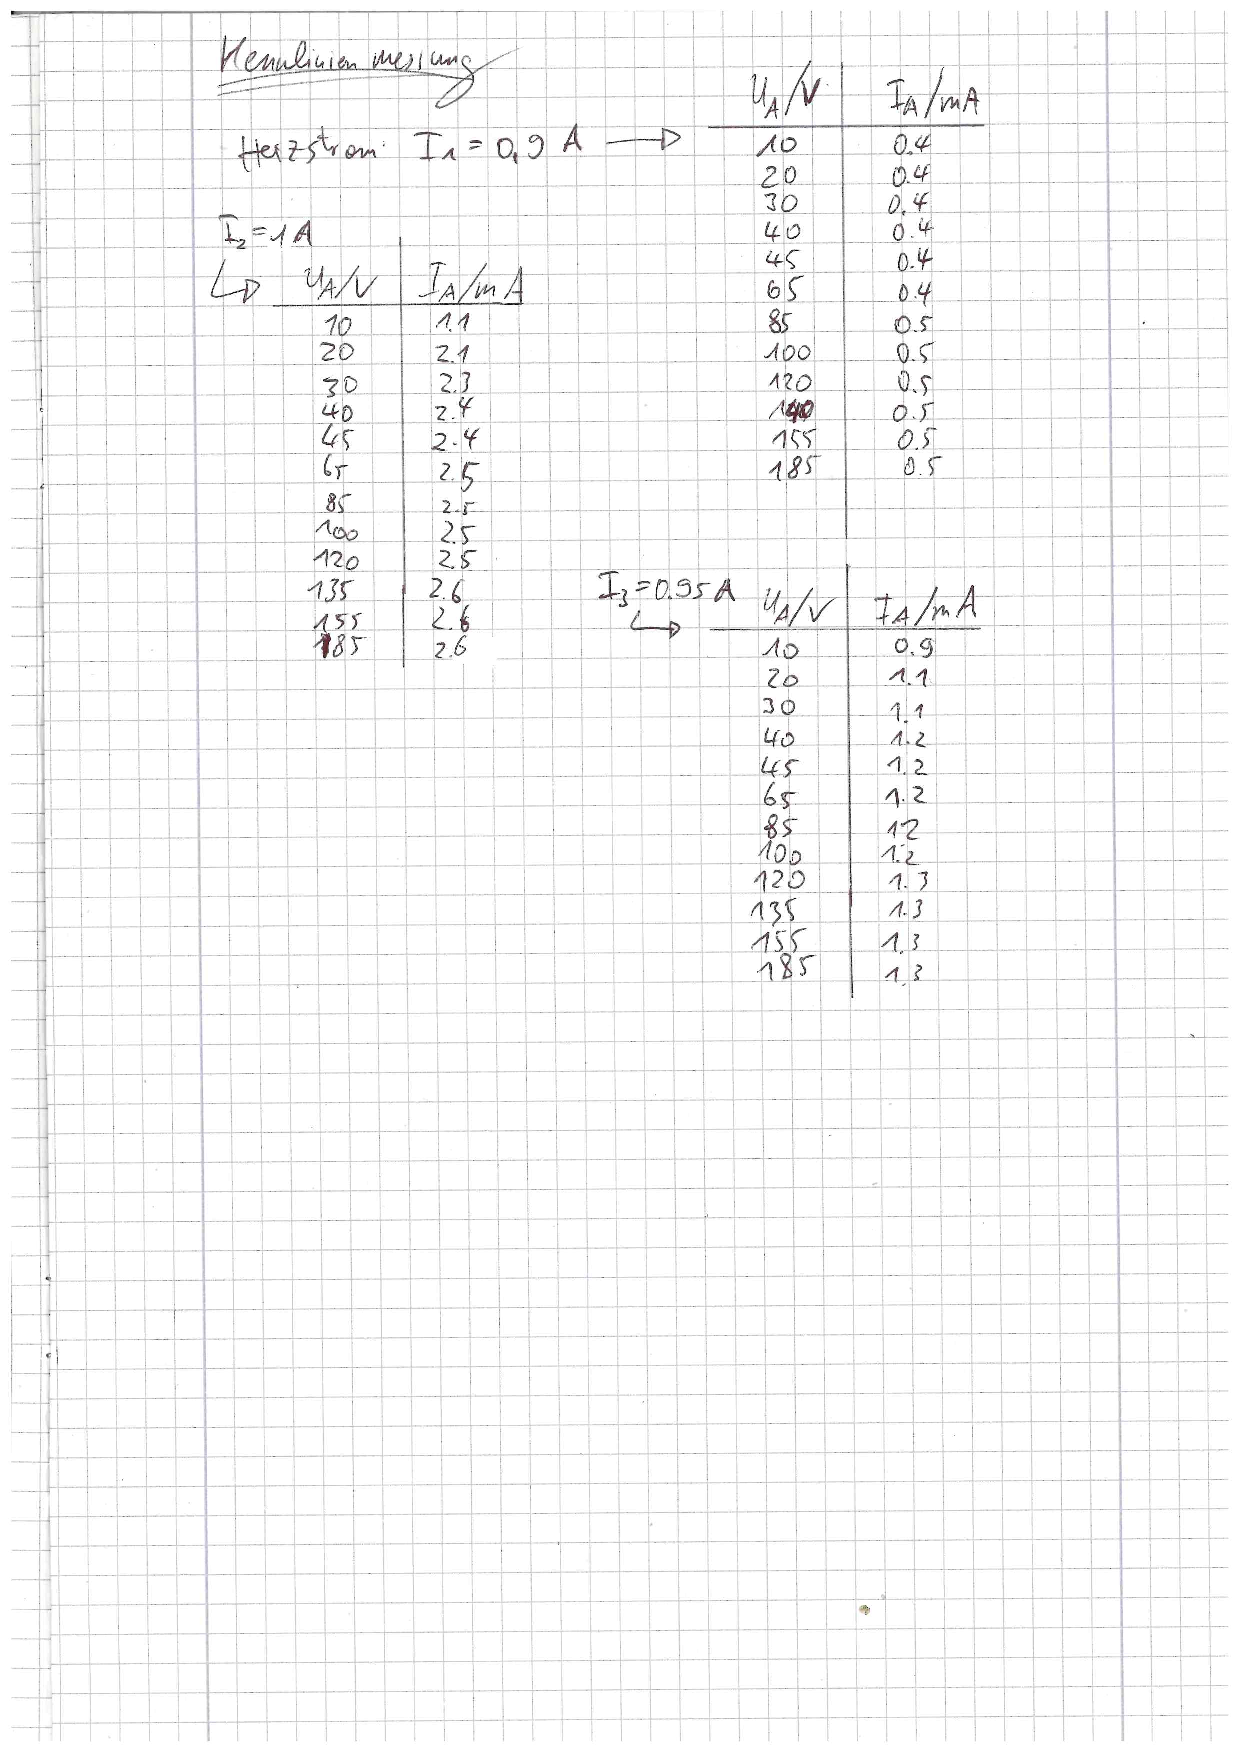
\includegraphics[width=0.8\textwidth]{messwerte/5.pdf}
  \caption{Fünfte Seite der Messwerte.}
  \label{fig:messwert5}
\end{figure}
